%%%%%%%%%%%%%%%%%%%%%%%%%%%%%%%%%%%%%%%%%%%%%%%%%%%%%%%%%%%%%%%%%%%%%%%%%%%%%%%%%%
\begin{frame}[fragile]\frametitle{}
\begin{center}
{\Large Support Vector Machine with Scikit-Learn}
\end{center}
\end{frame}

%%%%%%%%%%%%%%%%%%%%%%%%%%%%%%%%%%%%%%%%%%%%%%%%%%%%%%%%%%%%%%%%%%%%%%%%
\begin{frame}[fragile]\frametitle{Support Vector Machine}
\begin{lstlisting}
# Support Vector Machine
from sklearn import datasets
from sklearn import metrics
from sklearn.svm import SVC
# load the iris datasets
dataset = datasets.load_iris()
# fit a SVM model to the data
model = SVC()
model.fit(dataset.data, dataset.target)
print(model)
# make predictions
expected = dataset.target
predicted = model.predict(dataset.data)
# summarize the fit of the model
print(metrics.classification_report(expected, predicted))
print(metrics.confusion_matrix(expected, predicted))
\end{lstlisting}

{\tiny (Ref: Machine Learning Algorithm Recipes in scikit-learn - Jason Brownlee)}

\end{frame}

% %%%%%%%%%%%%%%%%%%%%%%%%%%%%%%%%%%%%%%%%%%%%%%%%%%%%%%%%%%%
% \begin{frame}[fragile]\frametitle{SVM Template Code}
% \begin{lstlisting}
% from sklearn import svm 

% #Assumed you have, X (predictor) and Y (target) for training data set and x_test(predictor) of test_dataset 

% model = svm.svc() 

% model.fit(X, y) 
% model.score(X, y) 

% #Predict Output 
% predicted= model.predict(x_test)
% \end{lstlisting}
% \end{frame}

% %%%%%%%%%%%%%%%%%%%%%%%%%%%%%%%%%%%%%%%%%%%%%%%%%%%%%%%%%%%%%%%%%%%%%%%%%%%%%%%%%%
% \begin{frame}[fragile]\frametitle{}
% \begin{center}
% {\Large Test case: Synthetic Data}
% \end{center}
% \end{frame}

% %%%%%%%%%%%%%%%%%%%%%%%%%%%%%%%%%%%%%%%%%%%%%%%%%%%%%%%%%%%
% \begin{frame}[fragile]\frametitle{Support Vector Machine Classifier}
% \begin{lstlisting}
% from sklearn.datasets.samples_generator import make_blobs

% X, y = make_blobs(n_samples=50, centers=2, random_state=0, cluster_std=0.60)

% xfit = np.linspace(-1, 3.5)
% plt.scatter(X[:, 0], X[:, 1], c=y, s=50, cmap='spring')

% # Draw three lines that couple separate the data
% for m, b, d in [(1, 0.65, 0.33), (0.5, 1.6, 0.55), (-0.2, 2.9, 0.2)]:
    % yfit = m * xfit + b
    % plt.plot(xfit, yfit, '-k')
    % plt.fill_between(xfit, yfit - d, yfit + d, edgecolor='none', color='#AAAAAA', alpha=0.4)

% plt.xlim(-1, 3.5);
% \end{lstlisting}
% \end{frame}

% %%%%%%%%%%%%%%%%%%%%%%%%%%%%%%%%%%%%%%%%%%%%%%%%%%%%%%%%%%%
% \begin{frame}[fragile]\frametitle{Support Vector Machine Classifier}
% \begin{center}
% 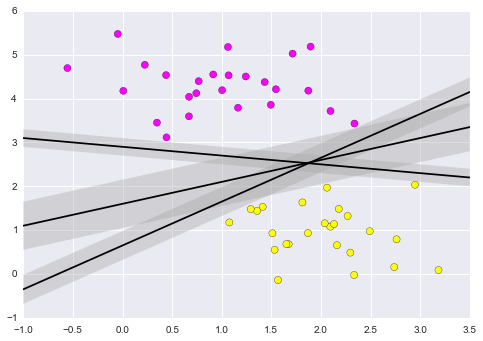
\includegraphics[width=0.8\linewidth,keepaspectratio]{svm1}
% \end{center}
% \end{frame}

% %%%%%%%%%%%%%%%%%%%%%%%%%%%%%%%%%%%%%%%%%%%%%%%%%%%%%%%%%%%
% \begin{frame}[fragile]\frametitle{}
% Fit the model
% \begin{lstlisting}
% from sklearn.svm import SVC

% clf = SVC(kernel='linear')
% clf.fit(X, y)
% \end{lstlisting}
% Plot the boundary:
% \begin{lstlisting}
% plt.scatter(X[:, 0], X[:, 1], c=y, s=50, cmap='spring')
% plot_svc_decision_function(clf)
% plt.scatter(clf.support_vectors_[:, 0], clf.support_vectors_[:, 1], s=200, facecolors='none');
% \end{lstlisting}
% \end{frame}

% %%%%%%%%%%%%%%%%%%%%%%%%%%%%%%%%%%%%%%%%%%%%%%%%%%%%%%%%%%%
% \begin{frame}[fragile]\frametitle{}
% Plotting function code:
% \begin{lstlisting}
% def plot_svc_decision_function(clf, ax=None):
    % """Plot the decision function for a 2D SVC"""
    % if ax is None:
        % ax = plt.gca()
    % x = np.linspace(plt.xlim()[0], plt.xlim()[1], 30)
    % y = np.linspace(plt.ylim()[0], plt.ylim()[1], 30)
    % Y, X = np.meshgrid(y, x)
    % P = np.zeros_like(X)
    % for i, xi in enumerate(x):
        % for j, yj in enumerate(y):
            % P[i, j] = clf.decision_function([xi, yj])
    % # plot the margins
    % ax.contour(X, Y, P, colors='k',
               % levels=[-1, 0, 1], alpha=0.5,
               % linestyles=['--', '-', '--'])
% \end{lstlisting}
% \begin{center}
% 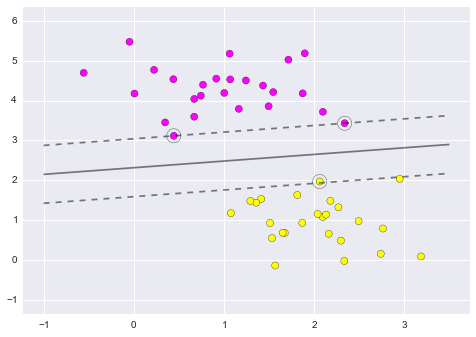
\includegraphics[width=0.3\linewidth,keepaspectratio]{svm2}
% \end{center}
% \end{frame}

% %%%%%%%%%%%%%%%%%%%%%%%%%%%%%%%%%%%%%%%%%%%%%%%%%%%%%%%%%%%
% \begin{frame}[fragile]\frametitle{Support Vector Machine with Kernels Classifier}
% \begin{itemize}
% \item Kernels are useful when the decision boundary is not linear. 
% \item A Kernel is some functional transformation of the input data. 
% \item SVMs ensure kernel calculations are efficient. 
% \item In the example below, a linear boundary is not useful in separating the groups of points.
% \end{itemize}
% \begin{lstlisting}
% from sklearn.datasets.samples_generator import make_circles
% X, y = make_circles(100, factor=.1, noise=.1)

% clf = SVC(kernel='linear').fit(X, y)
% plt.scatter(X[:, 0], X[:, 1], c=y, s=50, cmap='spring')
% plot_svc_decision_function(clf);
% \end{lstlisting}
% \begin{center}
% 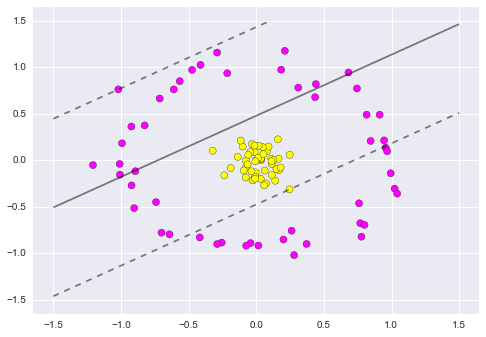
\includegraphics[width=0.3\linewidth,keepaspectratio]{svm3}
% \end{center}
% \end{frame}

% %%%%%%%%%%%%%%%%%%%%%%%%%%%%%%%%%%%%%%%%%%%%%%%%%%%%%%%%%%%
% \begin{frame}[fragile]\frametitle{Support Vector Machine with Kernels Classifier}
% A simple model that could be useful is a radial basis function:
% \begin{lstlisting}
% r = np.exp(-(X[:, 0] ** 2 + X[:, 1] ** 2))

% from mpl_toolkits import mplot3d

% def plot_3D(elev=30, azim=30):
    % ax = plt.subplot(projection='3d')
    % ax.scatter3D(X[:, 0], X[:, 1], r, c=y, s=50, cmap='spring')
    % ax.view_init(elev=elev, azim=azim)
% \end{lstlisting}
% \begin{center}
% 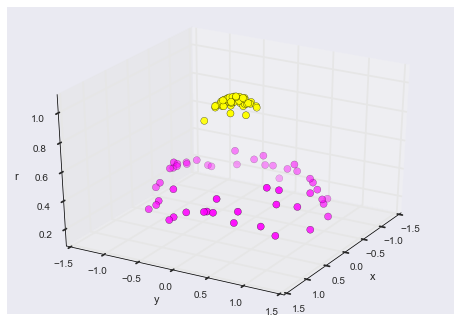
\includegraphics[width=0.35\linewidth,keepaspectratio]{svm4}
% \end{center}
% In three dimensions, there is a clear separation between the data.
% \end{frame}

% %%%%%%%%%%%%%%%%%%%%%%%%%%%%%%%%%%%%%%%%%%%%%%%%%%%%%%%%%%%
% \begin{frame}[fragile]\frametitle{Support Vector Machine with Kernels Classifier}
 % Run the SVM with the rbf kernel:
% \begin{lstlisting}
% clf = SVC(kernel='rbf')
% clf.fit(X, y)

% plt.scatter(X[:, 0], X[:, 1], c=y, s=50, cmap='spring')
% plot_svc_decision_function(clf)
% plt.scatter(clf.support_vectors_[:, 0], clf.support_vectors_[:, 1],
            % s=200, facecolors='none');
% \end{lstlisting}
% \begin{center}
% 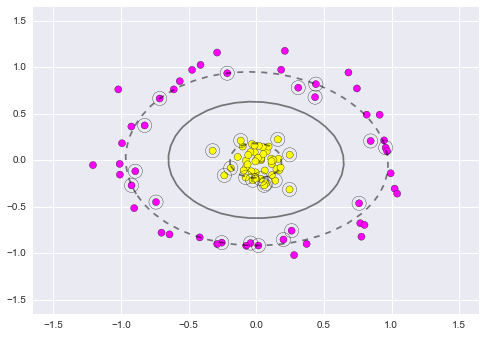
\includegraphics[width=0.5\linewidth,keepaspectratio]{svm5}
% \end{center}
% \end{frame}

% %%%%%%%%%%%%%%%%%%%%%%%%%%%%%%%%%%%%%%%%%%%%%%%%%%%%%%%%%%%%
% %\begin{frame}[fragile]\frametitle{Support Vector Machine Additional Notes}
% %\begin{itemize}
% %\item  When using an SVM you need to choose the right values for parameters such as c and gamma. 
% %\item Model validation can help to determine these optimal values by trial and error.
% %\item SVMs run in $O(n^3)$ performance.
% %%\item LinearSVC is scalable, SVC does not seem to be scalable.
% %\item For large data sets try transforming the data to a smaller space and use LinearSVC with rbf.
% %\end{itemize}
% %\end{frame}

% %%%%%%%%%%%%%%%%%%%%%%%%%%%%%%%%%%%%%%%%%%%%%%%%%%%%%%%%%%%%%%%%%%%%%%%%%%%%%%%%%%
% \begin{frame}[fragile]\frametitle{}
% \begin{center}
% {\Large Exercise: Ex6Data1}
% \end{center}
% \end{frame}


% %%%%%%%%%%%%%%%%%%%%%%%%%%%%%%%%%%%%%%%%%%%%%%%%%%%%%%%%%%%
% \begin{frame}[fragile]\frametitle{Exercise : Support Vector Machine}
% \begin{itemize}
% \item 2D example dataset which can be separated by a linear boundary
% \item Binary classification to be done using SVM
% \item Data file: ex6data1.mat
% \end{itemize}
% \begin{center}
% 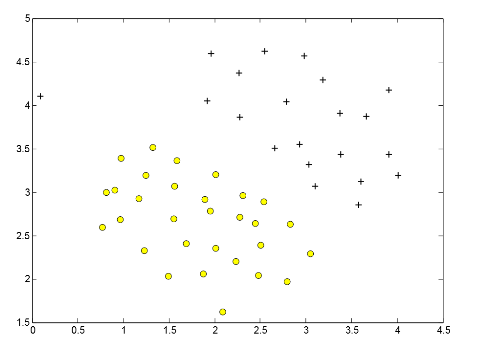
\includegraphics[width=0.6\linewidth,keepaspectratio]{svmex1}
% \end{center}
% \end{frame}

% %%%%%%%%%%%%%%%%%%%%%%%%%%%%%%%%%%%%%%%%%%%%%%%%%%%%%%%%%%%
% \begin{frame}[fragile]\frametitle{Exercise : Support Vector Machine}
% \begin{itemize}
% \item Try using different values of C (C controls penalty of mis-classified training examples)
% \item Large C tells SVM to classify all the examples correctly and vice versa.
% \end{itemize}
% $C=1$
% \begin{center}
% 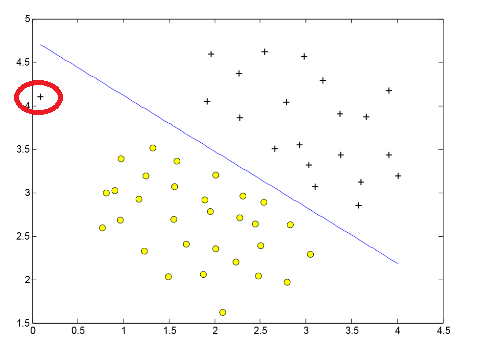
\includegraphics[width=0.6\linewidth,keepaspectratio]{svmex2}
% \end{center}
% \end{frame}

% %%%%%%%%%%%%%%%%%%%%%%%%%%%%%%%%%%%%%%%%%%%%%%%%%%%%%%%%%%%
% \begin{frame}[fragile]\frametitle{Exercise : Support Vector Machine}
% $C=100$
% \begin{center}
% 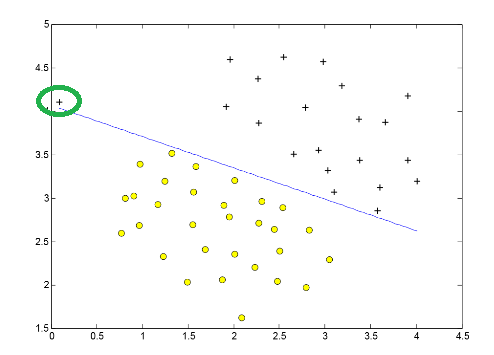
\includegraphics[width=0.6\linewidth,keepaspectratio]{svmex3}
% \end{center}
% \end{frame}

% %%%%%%%%%%%%%%%%%%%%%%%%%%%%%%%%%%%%%%%%%%%%%%%%%%%%%%%%%%%
% \begin{frame}[fragile]\frametitle{Exercise : Support Vector Machine}
% Load libraries and data
% \begin{lstlisting}
% import numpy as np
% import pandas as pd
% import matplotlib.pyplot as plt
% import seaborn as sb
% from scipy.io import loadmat

% raw_data = loadmat('data/ex6data1.mat')

% data = pd.DataFrame(raw_data['X'], columns=['X1', 'X2'])
% data['y'] = raw_data['y']

% positive = data[data['y'].isin([1])]
% negative = data[data['y'].isin([0])]
% \end{lstlisting}
% \end{frame}

% %%%%%%%%%%%%%%%%%%%%%%%%%%%%%%%%%%%%%%%%%%%%%%%%%%%%%%%%%%%
% \begin{frame}[fragile]\frametitle{Exercise : Support Vector Machine}
% Plot
% \begin{lstlisting}
% fig, ax = plt.subplots(figsize=(12,8))
% ax.scatter(positive['X1'], positive['X2'], s=50, marker='x', label='Positive')
% ax.scatter(negative['X1'], negative['X2'], s=50, marker='o', label='Negative')
% ax.legend()
% \end{lstlisting}
% \begin{center}
% 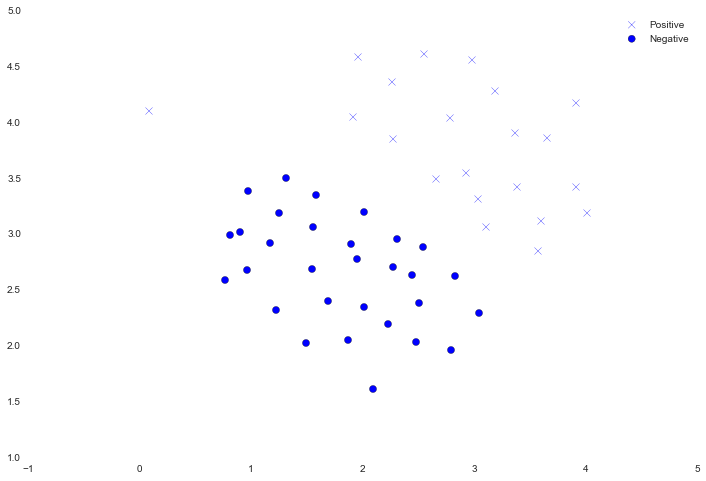
\includegraphics[width=0.6\linewidth,keepaspectratio]{svmex6}
% \end{center}
% \end{frame}

% %%%%%%%%%%%%%%%%%%%%%%%%%%%%%%%%%%%%%%%%%%%%%%%%%%%%%%%%%%%
% \begin{frame}[fragile]\frametitle{Exercise : Support Vector Machine}
% \begin{itemize}
% \item  Notice that one outlier positive example sits apart from the others
% \item The classes are still linearly separable but it's a very tight fit. 
% \item Going to train a linear support vector machine to learn the class boundary
% \item Use $svm.LinearSVC$ 
% \end{itemize}
% \end{frame}

% %%%%%%%%%%%%%%%%%%%%%%%%%%%%%%%%%%%%%%%%%%%%%%%%%%%%%%%%%%%
% \begin{frame}[fragile]\frametitle{Exercise : Support Vector Machine}
% Sklearn  svm.LinearSVC and $C=1$
% \begin{lstlisting}
% from sklearn import svm
% svc = svm.LinearSVC(C=1, loss='hinge', max_iter=1000)

% svc.fit(data[['X1', 'X2']], data['y'])

% svc.score(data[['X1', 'X2']], data['y'])
% \end{lstlisting}
% 0.98039215686274506
% \end{frame}

% %%%%%%%%%%%%%%%%%%%%%%%%%%%%%%%%%%%%%%%%%%%%%%%%%%%%%%%%%%%
% \begin{frame}[fragile]\frametitle{Exercise : Support Vector Machine}
% With $C=100$
% \begin{lstlisting}
% svc2 = svm.LinearSVC(C=100, loss='hinge', max_iter=1000)
% svc2.fit(data[['X1', 'X2']], data['y'])
% svc2.score(data[['X1', 'X2']], data['y'])
% \end{lstlisting}
% 1.0
% \end{frame}

% %%%%%%%%%%%%%%%%%%%%%%%%%%%%%%%%%%%%%%%%%%%%%%%%%%%%%%%%%%%
% \begin{frame}[fragile]\frametitle{Exercise : Support Vector Machine}
% \begin{itemize}
% \item  Got a perfect classification of the training data, 
% \item However by increasing the value of C, the decision boundary is no longer a natural fit for the data. 
% \item Plot confidence level for each class prediction
% \item Its a function of the points distance from the hyper-plane.
% \item Visualization could be subtle but lets try.
% \end{itemize}
% \end{frame}

% %%%%%%%%%%%%%%%%%%%%%%%%%%%%%%%%%%%%%%%%%%%%%%%%%%%%%%%%%%%
% \begin{frame}[fragile]\frametitle{Exercise : Support Vector Machine}
% Confidence $C=1$
% \begin{lstlisting}
% data['SVM 1 Confidence'] = svc.decision_function(data[['X1', 'X2']])

% fig, ax = plt.subplots(figsize=(12,8))
% ax.scatter(data['X1'], data['X2'], s=50, c=data['SVM 1 Confidence'], cmap='seismic')
% ax.set_title('SVM (C=1) Decision Confidence')
% \end{lstlisting}
% \begin{center}
% 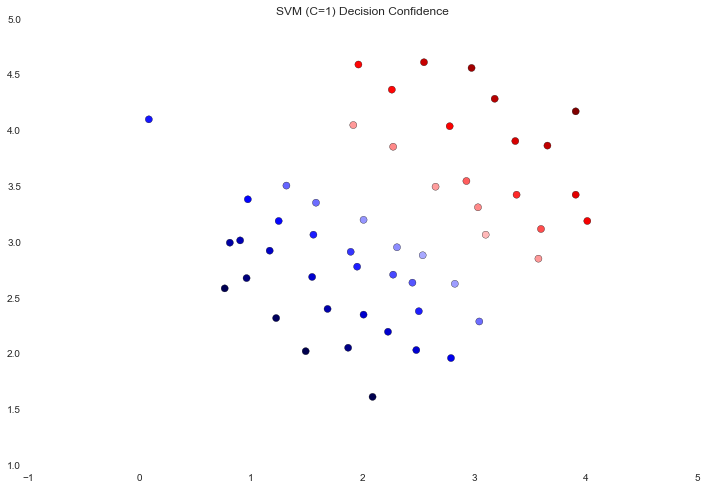
\includegraphics[width=0.6\linewidth,keepaspectratio]{svmex7}
% \end{center}
% Color strength is confidence value. Look at the outlier classification as well.
% \end{frame}


% %%%%%%%%%%%%%%%%%%%%%%%%%%%%%%%%%%%%%%%%%%%%%%%%%%%%%%%%%%%
% \begin{frame}[fragile]\frametitle{Exercise : Support Vector Machine}
% Confidence $C=100$
% \begin{lstlisting}
% data['SVM 2 Confidence'] = svc2.decision_function(data[['X1', 'X2']])

% fig, ax = plt.subplots(figsize=(12,8))
% ax.scatter(data['X1'], data['X2'], s=50, c=data['SVM 2 Confidence'], cmap='seismic')
% ax.set_title('SVM (C=100) Decision Confidence')
% \end{lstlisting}
% \begin{center}
% 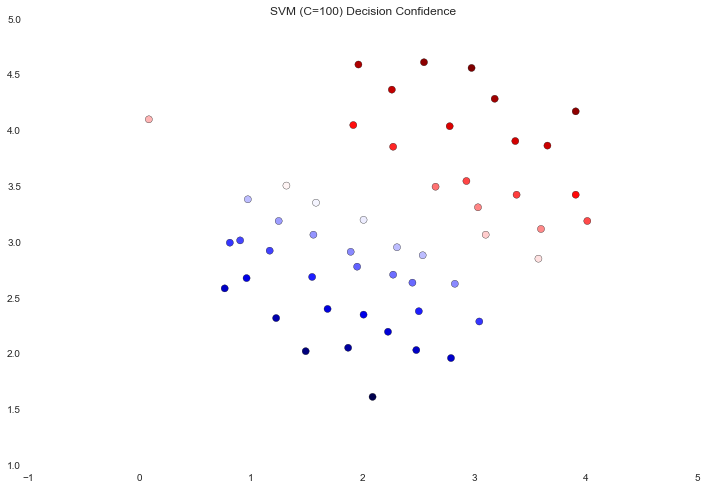
\includegraphics[width=0.6\linewidth,keepaspectratio]{svmex8}
% \end{center}
% Color strength is confidence value. Look at the outlier classification as well.
% \end{frame}

% %%%%%%%%%%%%%%%%%%%%%%%%%%%%%%%%%%%%%%%%%%%%%%%%%%%%%%%%%%%
% \begin{frame}[fragile]\frametitle{Exercise : Support Vector Machine as Spam Classifier}
% Non Linear Kernel for example data-set 2
% \begin{center}
% 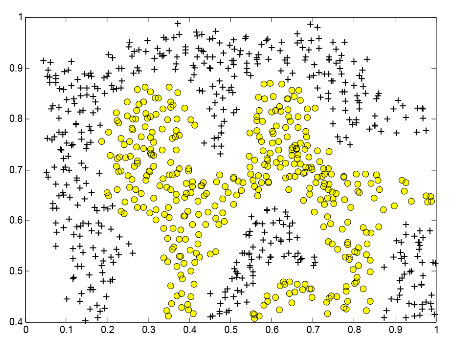
\includegraphics[width=0.6\linewidth,keepaspectratio]{svmex4}
% \end{center}
% \end{frame}

% %%%%%%%%%%%%%%%%%%%%%%%%%%%%%%%%%%%%%%%%%%%%%%%%%%%%%%%%%%%
% \begin{frame}[fragile]\frametitle{Exercise : Support Vector Machine as Spam Classifier}
% Result for example data-set 2 could be:
% \begin{center}
% 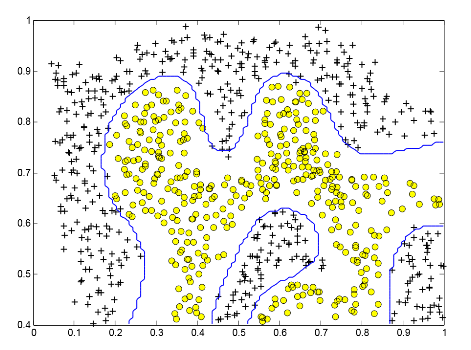
\includegraphics[width=0.6\linewidth,keepaspectratio]{svmex5}
% \end{center}
% \end{frame}
% %
% %%%%%%%%%%%%%%%%%%%%%%%%%%%%%%%%%%%%%%%%%%%%%%%%%%%%%%%%%%%%
% %\begin{frame}[fragile]\frametitle{Exercise : Support Vector Machine}
% %Non Linear SVM using Gaussian Kernel
% %\begin{itemize}
% %\item Sklearn has ready Gaussian function
% %\item Lets write on our own
% %\end{itemize}
% %\begin{lstlisting}
% %def gaussian_kernel(x1, x2, sigma):
% %    return np.exp(-(np.sum((x1 - x2) ** 2) / (2 * (sigma ** 2))))
% %    
% %x1 = np.array([1.0, 2.0, 1.0])
% %x2 = np.array([0.0, 4.0, -1.0])
% %sigma = 2
% %
% %gaussian_kernel(x1, x2, sigma)
% %
% %0.32465246735834974
% %\end{lstlisting}
% %\end{frame}
% %
% %%%%%%%%%%%%%%%%%%%%%%%%%%%%%%%%%%%%%%%%%%%%%%%%%%%%%%%%%%%
% \begin{frame}[fragile]\frametitle{Exercise : Support Vector Machine}
% \begin{itemize}
% \item Its a similarity/distance value between pair of examples, parametrized by sigma.
% \item Lower value, points are apart.
% \item Lets use this on another non linearly separable dataset
% \end{itemize}

% \end{frame}

% %%%%%%%%%%%%%%%%%%%%%%%%%%%%%%%%%%%%%%%%%%%%%%%%%%%%%%%%%%%%%%%%%%%%%%%%%%%%%%%%%%
% \begin{frame}[fragile]\frametitle{}
% \begin{center}
% {\Large Exercise: Ex6Data2}
% \end{center}
% \end{frame}

% %%%%%%%%%%%%%%%%%%%%%%%%%%%%%%%%%%%%%%%%%%%%%%%%%%%%%%%%%%%
% \begin{frame}[fragile]\frametitle{Exercise : Support Vector Machine}
% Load data
% \begin{lstlisting}
% raw_data = loadmat('data/ex6data2.mat')

% data = pd.DataFrame(raw_data['X'], columns=['X1', 'X2'])
% data['y'] = raw_data['y']

% positive = data[data['y'].isin([1])]
% negative = data[data['y'].isin([0])]
% \end{lstlisting}
% \end{frame}

% %%%%%%%%%%%%%%%%%%%%%%%%%%%%%%%%%%%%%%%%%%%%%%%%%%%%%%%%%%%
% \begin{frame}[fragile]\frametitle{Exercise : Support Vector Machine}
% Plot
% \begin{lstlisting}
% fig, ax = plt.subplots(figsize=(12,8))
% ax.scatter(positive['X1'], positive['X2'], s=30, marker='x', label='Positive')
% ax.scatter(negative['X1'], negative['X2'], s=30, marker='o', label='Negative')
% ax.legend()
% \end{lstlisting}
% \begin{center}
% 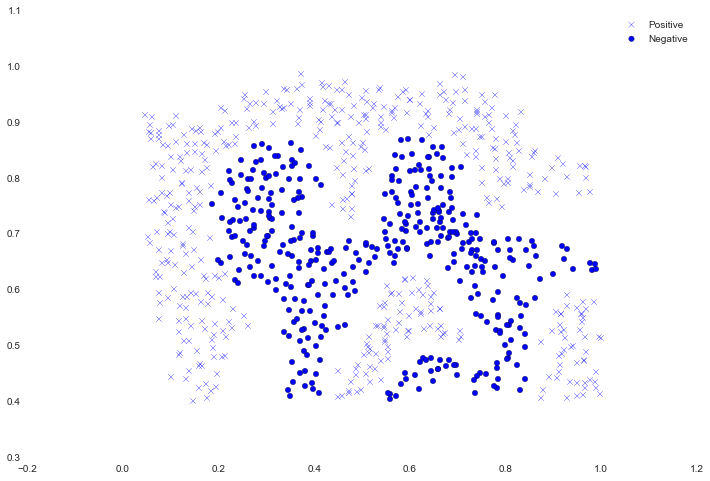
\includegraphics[width=0.6\linewidth,keepaspectratio]{svmex9}
% \end{center}
% \end{frame}

% %%%%%%%%%%%%%%%%%%%%%%%%%%%%%%%%%%%%%%%%%%%%%%%%%%%%%%%%%%%
% \begin{frame}[fragile]\frametitle{Exercise : Support Vector Machine}
% Build a support vector machine classifier using the built-in RBF kernel (default is ``kernel='rbf'''), Radial Basis Function.
% \begin{lstlisting}
% svc = svm.SVC(C=100, gamma=10, probability=True)

% svc.fit(data[['X1', 'X2']], data['y'])
% svc.score(data[['X1', 'X2']], data['y'])
% \end{lstlisting}
% 0.9698725376593279
% \end{frame}


